%%%%%%%%%%%%%%%%%%%%%%%%%%%%%%%%%%%%%%%%%%%%%%%%%%%%%%%%%%%%%%%%%%%%%%%%%%%%%%%%%%%%%%%%%%%%%
%%									Chapitre 2												%
%%%%%%%%%%%%%%%%%%%%%%%%%%%%%%%%%%%%%%%%%%%%%%%%%%%%%%%%%%%%%%%%%%%%%%%%%%%%%%%%%%%%%%%%%%%%%

\chapter{Détection de Nouveauté}
	\citationChap{
		D'abord, j'observe les êtres humains car je les aime bien. J'enregistre dans ma tête tout ce que j'ai remarqué, et ensuite, avec les souvenirs de ce que j'ai vu, je dessine.
	}{Hayao Miyazaki}
	\minitoc
	\newpage

%%%%%%%%%%%%%%%%%%%%%%%%%%%%%%%%%%%%%%%%%%%%%%%%%%%%%%%%%%%%%%%%%%%%%%%%%%%%%%%%%%%%%%%%%%%%%



% Début du chapitre
			
	\section{Introduction}
	\section{Modèles Neuronaux}
	\subsection{Cartes Auto-Organisatrices}
	\subsection{Gaz Neuronaux en Croissance}

	\newpage
	\section{Traitements des images}\label{sec:images}

	Il existe de nombreuses possibilités différentes pour apprendre des images avec la quantification vectorielle, dû au grand nombre de façons de découper une image en vecteurs d'entrée. Pour présenter les alternatives que l'on a notre disposition pour apprendre des images, on peut considérer deux extrême : apprendre l'image en entier ou apprendre chaque pixel individuellement. Le premier cas peut sembler absurde dans le cas d'une seule image (une base de données d'un seul élément), mais peut présenter un intérêt lorsque l'on considère une suite d'images par exemple. Dans cet exemple, l'environnement appris serait défini par l'entièreté de ce que voit le capteur et tous les changements, où qu'ils soient dans l'image, auraient de l'importance.

	Le second extrême est l'apprentissage au niveau du pixel. Dans cette approche on prend chaque pixel individuel comme un vecteur d'entrée, ce qui rendrait l'espace d'entrée unidimensionnel pour une image en niveau de gris (ou tridimensionnel si l'image est en couleur, plus de détails dans la section \ref{sec:img:colors}). Sur un plan conceptuel, cette option considère qu'une image est définie uniquement par les couleurs ou luminosités présentes, peu importe leur positions dans celle-ci. Ce qui peut être utile dans certains cas particuliers, mais n'est pas adapté à ce que l'on souhaite faire dans cette thèse.

	Il existe un très grand nombre d'autres découpages possibles entre ces deux extrêmes, chacun représentant une certaine façon de considérer une image, et par conséquent la différence ou similarité entre deux images. C'est à dire que les différences qui vont apparaître en comparant deux images seront différentes et dépendront de la façon dont celles-ci seront représentées.

	Il est important donc de considérer le contexte de nos travaux pour définir la façon de représenter une image, notre application cible étant la detection de nouveauté. Dans ce contexte, nous considérons qu'une image est une combinaison de nombreux éléments plus petits. Par exemple, une photographie d'un lac de montagne \ref{fig:img:nino} peut être décrite comme étant la combinaison d'un élément de lac (avec sa couleur, bleu sombre et sa texture uniforme), d'un élément de plaine herbeuse (verte et uniforme), d'éléments rocailleux qui sont gris et soit uniformes (dans le premier plan) soit plus contrastés en se combinant avec la verdure de la végétation (dans les bords de l'image), et ainsi de suite. Ce genre de découpage "sémantique" de l'image est ce qui permet la détection de nouveauté  de fonctionner, car dans notre cas la nouveauté est par définition ce que n'est pas déjà dans l'image et donc ne faisant pas partie de ces éléments au sens large. Pour regrouper les parties d'une images appartenant au même élément, il est nécessaire d'avoir une information mise en contexte (un pixel seul ne suffit généralement pas à savoir à quel élément il appartient dans l'image), ce qui implique que les pixels doivent être pris dans leurs environnements locaux pour conserver l'information de voisinage comme la texture par exemple. Nous avons donc choisi de découper l'image en plus petites images à la façon d'une mosaique, que nous appellerons des imagettes. Ces imagettes (d'une taille arbitraire en hauteur et largeur) conservent l'environnement local tout en étant suffisament petites pour être précises dans l'espace (une imagette ne représentant qu'une partie d'un élément et non pas regroupant plusieurs éléments, ce qui réduirait sa capacité de généralisation), et permettre d'avoir une base d'apprentissage assez étoffée pour tirer parti des propriétés de nos modèles de quantification vectorielle et de leur topologie. La partie pratique de l'apprentissage d'une image, sa représentation et sa reconstruction sont abordés dans la section suivante \ref{sec:img:compression}.


	\begin{figureth}
		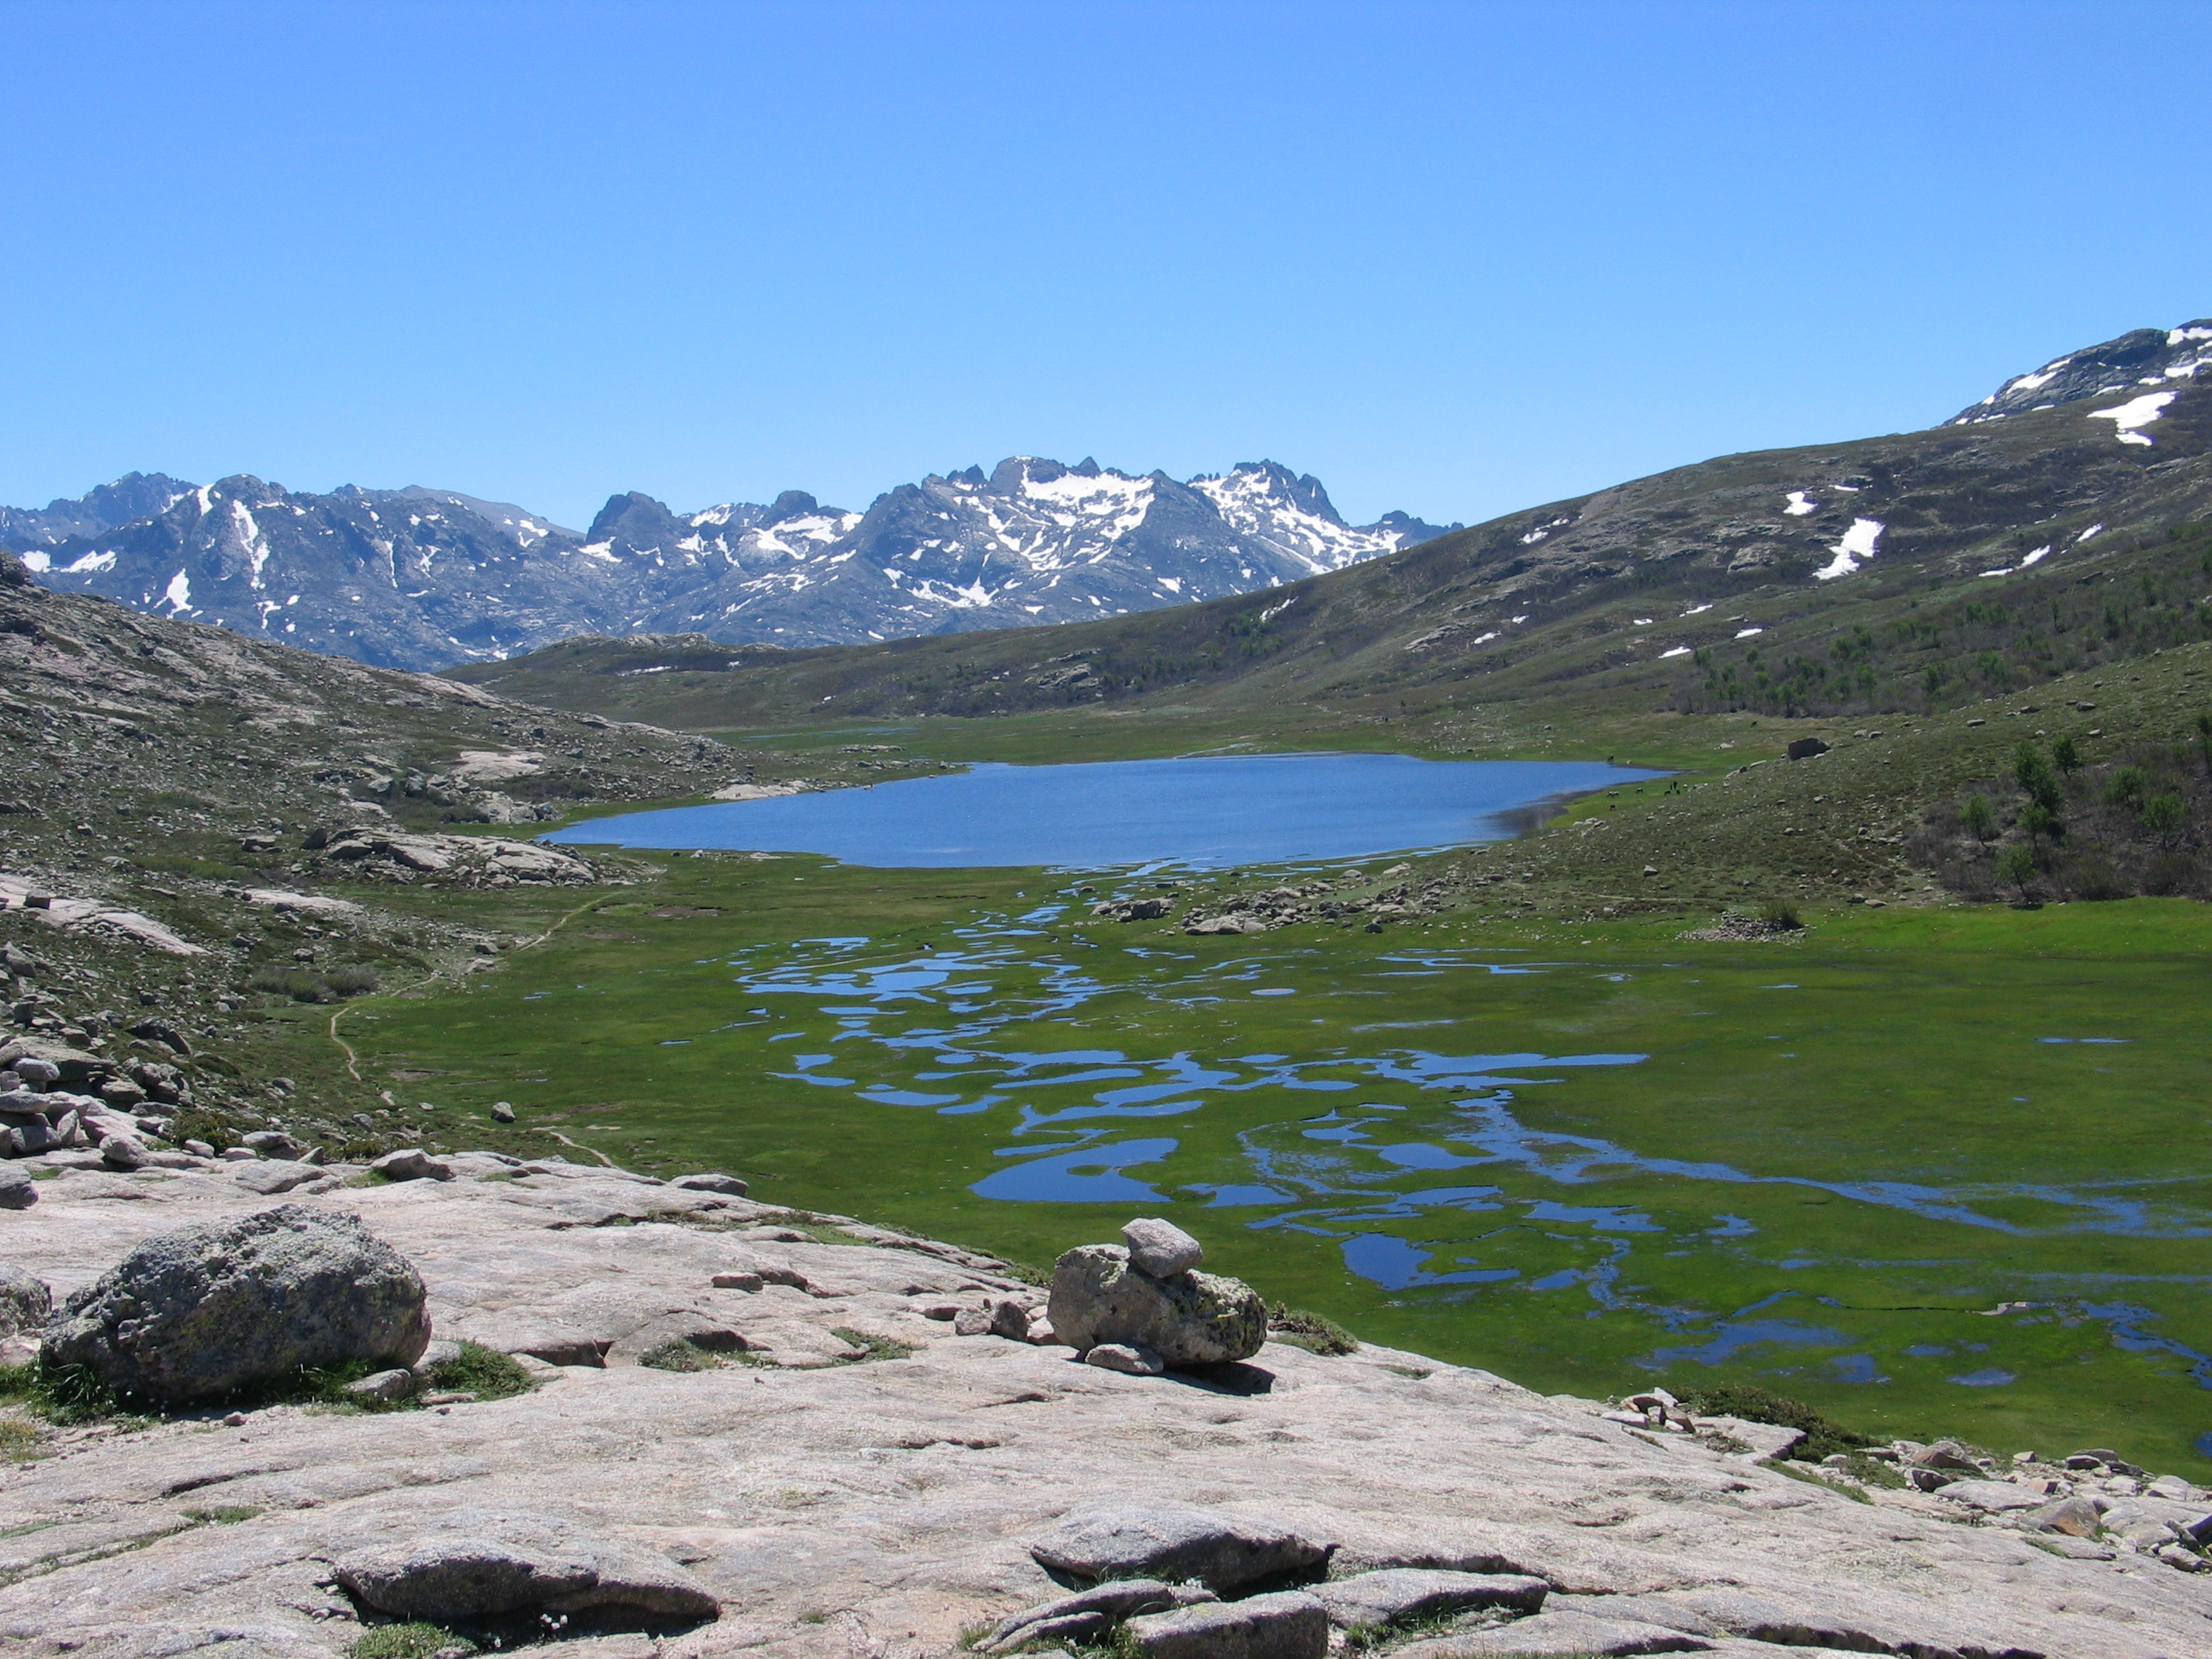
\includegraphics[width=\linewidth]{Lac_de_Nino}
		\caption[Lac de Nino]{Exemple d'image comportant plusieurs éléments notables tels qu'un lac (bleu sombre et uniforme), une plaine herbeuse (verte et uniforme), d'éléments rocailleux qui sont gris et soit uniformes (dans le premier plan) soit plus contrastés en se combinant avec la verdure de la végétation (dans les bords de l'image), et ainsi de suite.}\label{fig:img:nino}
	\end{figureth}

	\subsection{Apprentissage et reconstruction}\label{sec:img:compression}
	\subsubsection{Apprentissage}
	La première étape nécessaire à l'apprentissage est la constitution de la base d'apprentissage à partir de l'image. L'utilisation de modèles de quantification vectorielle établissent la première contrainte pour le découpage : les imagettes doivent être d'une taille fixe. En effet il est nécessaire pour les SOM comme pour les GNG et leurs variantes que tous les vecteurs d'entrées soient de la même longueur pour que le calcul de distance avec les neurones fonctione, qu'ils représentent correctement les entrées qui leurs sont attachées.

	Nous avons également choisi de limiter nos tailles d'imagettes à des valeurs carrées, pour des raisons de simplicité. Il est possible que des imagettes plus larges que hautes ou plus hautes que larges représentent mieux les éléments de l'image que l'on apprend. Cependant ce serait une préférence spécifique à chaque image et peu généralisable, car si on effectue par exemple une rotation de 90° de l'image, la préférence s'inversera. L'inversement des tailles dans les imagettes carrées ne changeant rien, elles sont pour leur part insensibles aux rotations discrètes de l'image (par pas de 90°).

	Dans la version classique, le découpage de l'image se fait en mosaique, sans superpositions entre les imagettes. C'est à dire que chaque pixel n'appartient qu'à une seule imagette. Le processus est montré sur la figure \ref{fig} Si les dimensions de l'images ne sont pas un multiple de la taille des imagettes, les pixels en trop sont simplement rognés par la droite et par le bas, car en général ils ne contiennent pas beaucoup d'informations.

	\begin{figureth}
		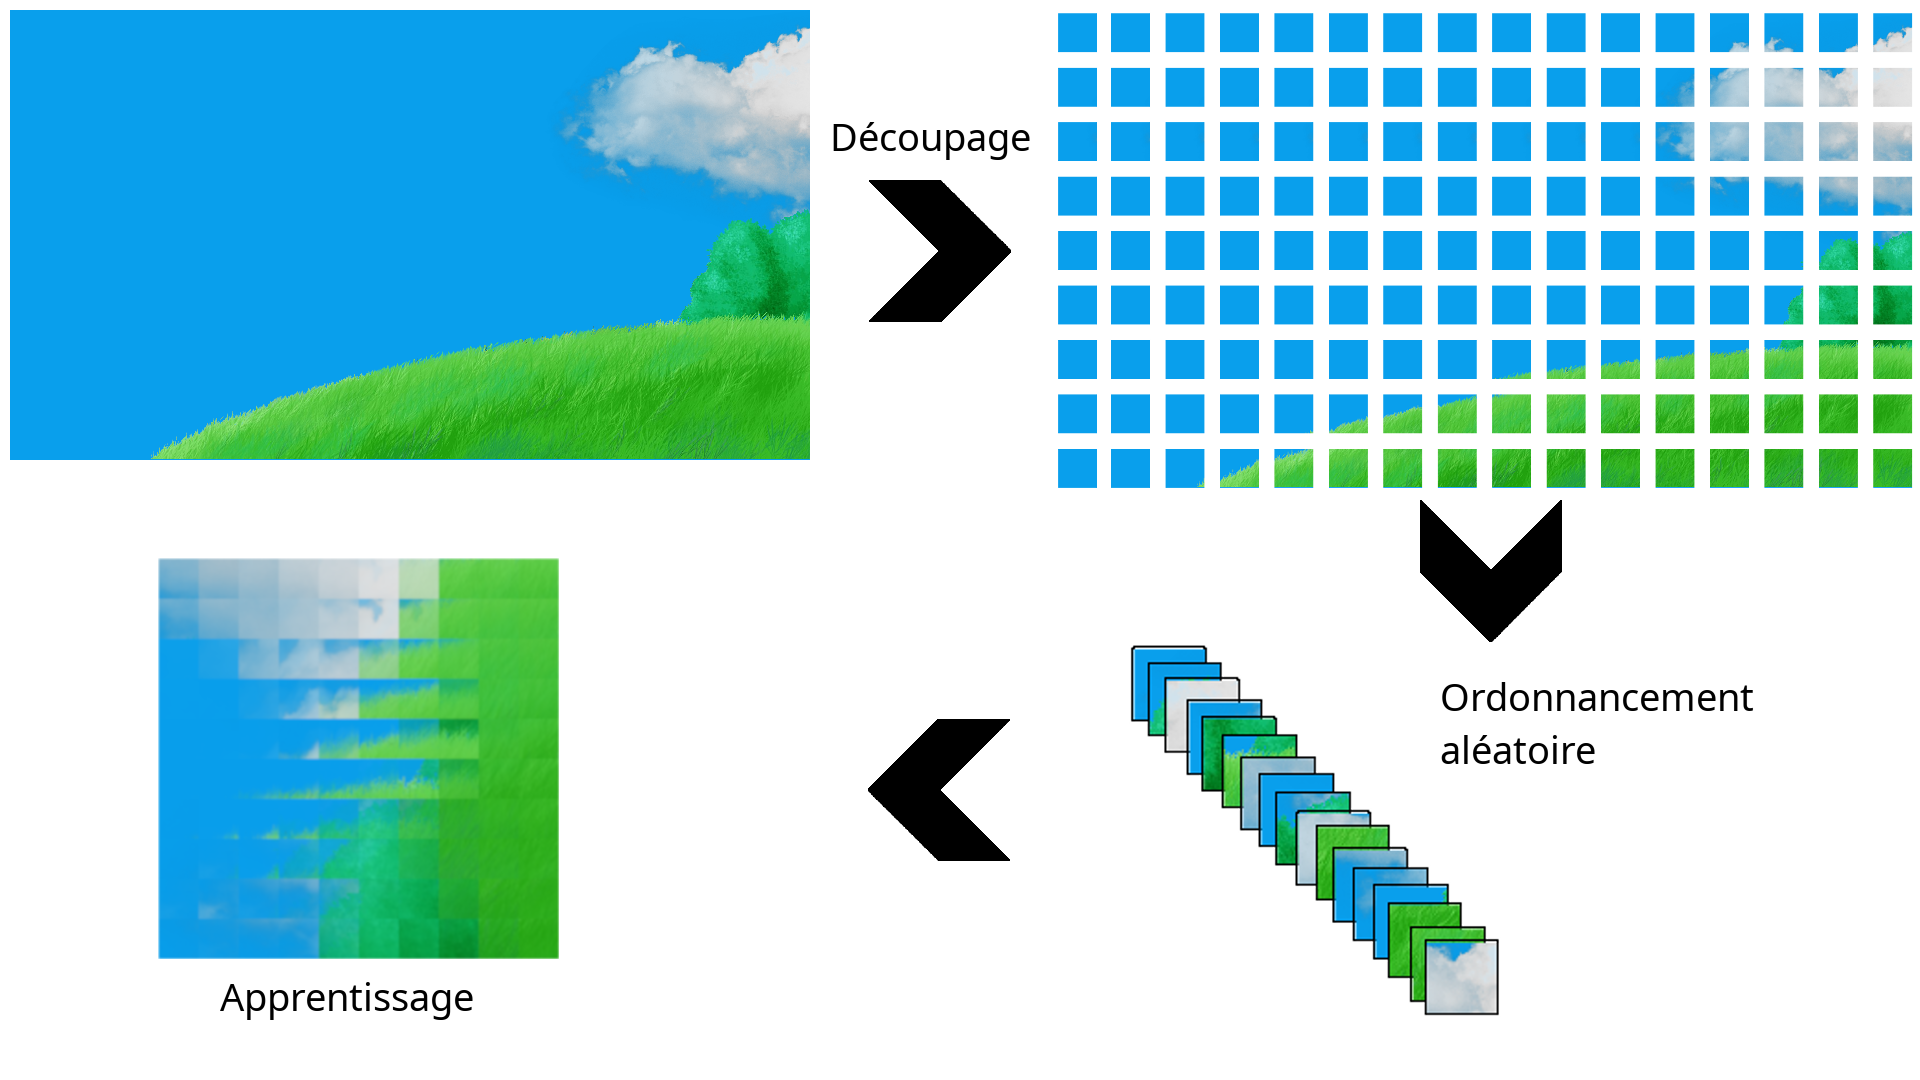
\includegraphics[width=\linewidth]{image_representation}
		\caption[Représentation d'une image]{Illustration du processus de représentation et d'apprentissage d'une image par une SOM.}\label{fig:img:rep}
	\end{figureth}

	\subsubsection{Reconstruction}

	Une fois l'apprentissage terminé, il y a deux résultats. Le premier est le modèle entrainé avec les différents poids des neurones codant une imagette représentante du cluster d'imagettes associé à ce neurone. Le second, facultatif, est la liste pour chaque imagette de l'image l'indexe du neurone le plus proche de celle-ci, qui pourra être utilisée pour la reconstruction de l'image d'apprentissage.  

	Pour reconstruire une image à partir de la liste des indexes de BMU, il suffit de remplacer chaque index par le vecteur prototype du neurone auquel il correspond. Ces vecteurs prototypes devront être réassemblés en imagettes (dans un tableau à 2 dimensions à la place d'un vecteur à une dimension), et placées à la bonne position pour reformer l'image.

	Il est aussi possible de reconstruire une image qui n'a pas été apprise. Pour cela il faut créer la liste d'indexes de neurones des imagettes de la nouvelle image, et de reconstruire ensuite l'image par le même procédé que montré précédemment. Il faut noter que l'image que l'on souhaite reconstituer doit être proche de l'image apprise pour avoir un résultat correct.

	\begin{figureth}
		\begin{subfigureth}{\textwidth}
			\includegraphics[width=\linewidth]{triangle/Image_compression2}
		\end{subfigureth}
		\begin{subfigureth}{\textwidth}
			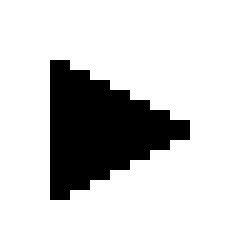
\includegraphics[width=0.2\linewidth]{triangle/triangle_original}\hfill
			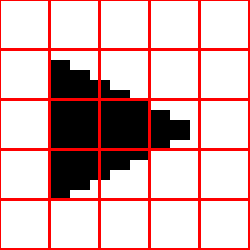
\includegraphics[width=0.2\linewidth]{triangle/triangle_grid}\hfill
			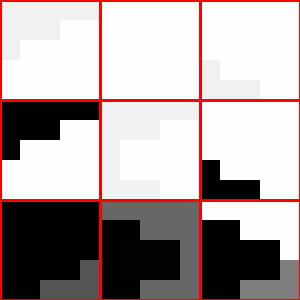
\includegraphics[width=0.2\linewidth]{triangle/som}\hfill
			
\includegraphics[width=0.2\linewidth]{triangle/triangle}
		\end{subfigureth}
		\caption[Compression et décompression d'image]{Schéma simplifié du processus de compression et de reconstruction d'une image, avec ici seulement 9 neurones et 25 imagettes.}\label{fig:img:comp_ex}
	\end{figureth}

	\subsection{La gestion des canaux (couleurs)}\label{sec:img:colors}

	Nous avons jusque là vu comment apprendre une image ayant une seule valeur par pixel (soit des images en nuances de gris). Cependant la majorité des dispositifs de capture actuels fournissent des images en couleur, c'est à dire trois canaux. Nous allons voir dans cette section comment transposer l'apprentissage, la compression et la reconstruction à des images à un nombre arbitraire de canaux par pixels.

	Une approche possible serait de séparer l'image par composante (une image RVB par exemple donnerait trois images en niveau de gris, une R, une V et une B). Deux options s'offrent ensuite à nous. Soit utiliser une seule SOM pour apprendre toutes les images ainsi extraites en espérant que les différentes formes présentes dans chaque composante soient assez similaires entre elles pour ne pas trop surcharger la SOM de données (car on vient de multiplier la taille de notre base d'apprentissage par le nombre de canaux), et que ces données restent assez cohérentes dans l'espace d'entrée pour que la réduction dimensionnelle se fasse correctement. Soit utiliser une SOM par composante pour apprendre chaque canal séparément, et de regrouper ensuite les différents canaux reconstitués en une image couleur. 
	
	Cependant ces deux approches ont un défaut majeur pour la compression d'images (ainsi que la détection de nouveauté par conséquent), c'est la création d'aberrations chromatiques dans l'image reconstituée. En effet, les canaux étant appris séparément avant d'être recombinés, la reconstruction peut donner pour certains pixels des teintes de couleurs qui n'existaient pas dans l'image de base, et très saillants visuellement. Par exemple un pixel blanc dans l'image d'entrée (avec une forte composante R, V et B), lorsque reconstitué par la SOM peut être bien reconstitué dans deux composantes (V et B par exemple), et mal reconstitué dans la troisième (R) avec une valeur beaucoup plus faible que dans l'image de base (cela arrive car notre calcul de distance minimise ). Par conséquent ce pixel aura une couleur turquoise dans l'image reconstituée à la place de blanc. Ce genre d'erreur est particulièrement mauvaise, car le résultat de la reconstruction minimise bien de façon optimale la distance avec l'image de base, et ce n'est que visuellement que les changements de teintes sont apparents et dégradent qualitativement l'image plus que ce que l'erreur mesurée ne laisse penser.

	Une meilleure approche consiste à inclure tous les canaux directements dans les imagettes. Chaque imagette devient donc une imagette en couleur, et sa taille augmente donc en conséquence. Une imagette de 10 par 10 pixels par exemple qui donnerait un vecteur prototype de taille 100, passe à 300 avec les trois couleurs. L'apprentissage et la reconstruction se déroulent de la même manière que dans la SOM classique. Il faut aussi noter que l'ordre n'a pas d'importance dans les vecteurs prototypes, on peut arranger les valeurs en RGBRGBRGB tout comme RRRGGGBBB sans que cela ne change le résultat, le calcul de distance euclidienne étant indépendant de l'ordre des coordonnées.

	\begin{figureth}
		\begin{subfigureth}{0.48\textwidth}
			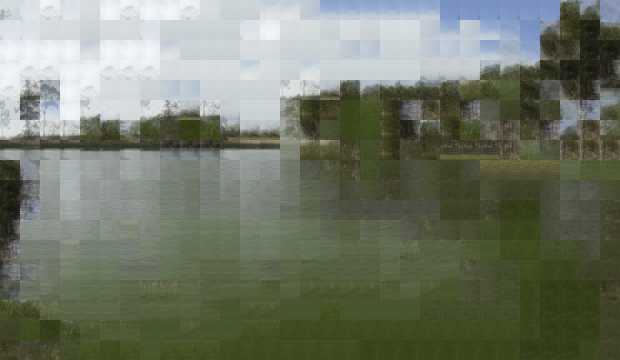
\includegraphics[width=\linewidth]{fusioned_color}\caption{Couleurs fusionnées}	
		\end{subfigureth}
		\begin{subfigureth}{0.48\textwidth}
			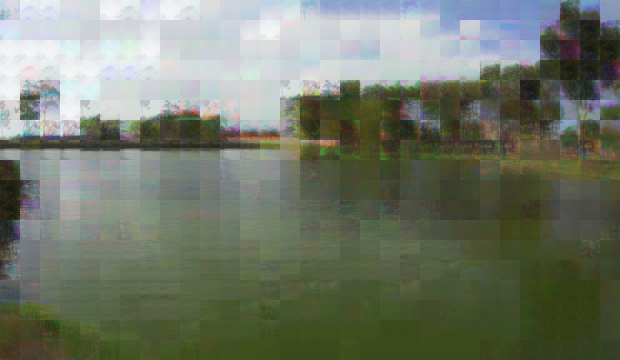
\includegraphics[width=\linewidth]{separated_colors}\caption{Couleurs séparées}	
		\end{subfigureth}
		\caption[Représentation d'une image]{Comparaison entre une image avec des couleurs fusionnées et la même image avec des couleurs séparées qui présente des artefacts visuels.}\label{fig:img:rep}
	\end{figureth}

	\newpage
	\section{Détection de nouveauté}

	Nous avons, à partir des différents principes, objectifs et fonctionnements définis dans les sections précédentes, développé deux processus de détection de nouveauté complémentaires. Nous présentons ces deux méthodes dans cette partie. La première est basée sur la propriété de quantification vectorielle de nos modèles pour trouver de la nouveauté précisément dans des images. La seconde est basée sur la topologie de nos modèles pour détecter de la nouveauté, qui donne des résultats moins précis, mais aussi moins bruités.

	\subsection{Détection avec quantification vectorielle}

	\begin{figureth}
		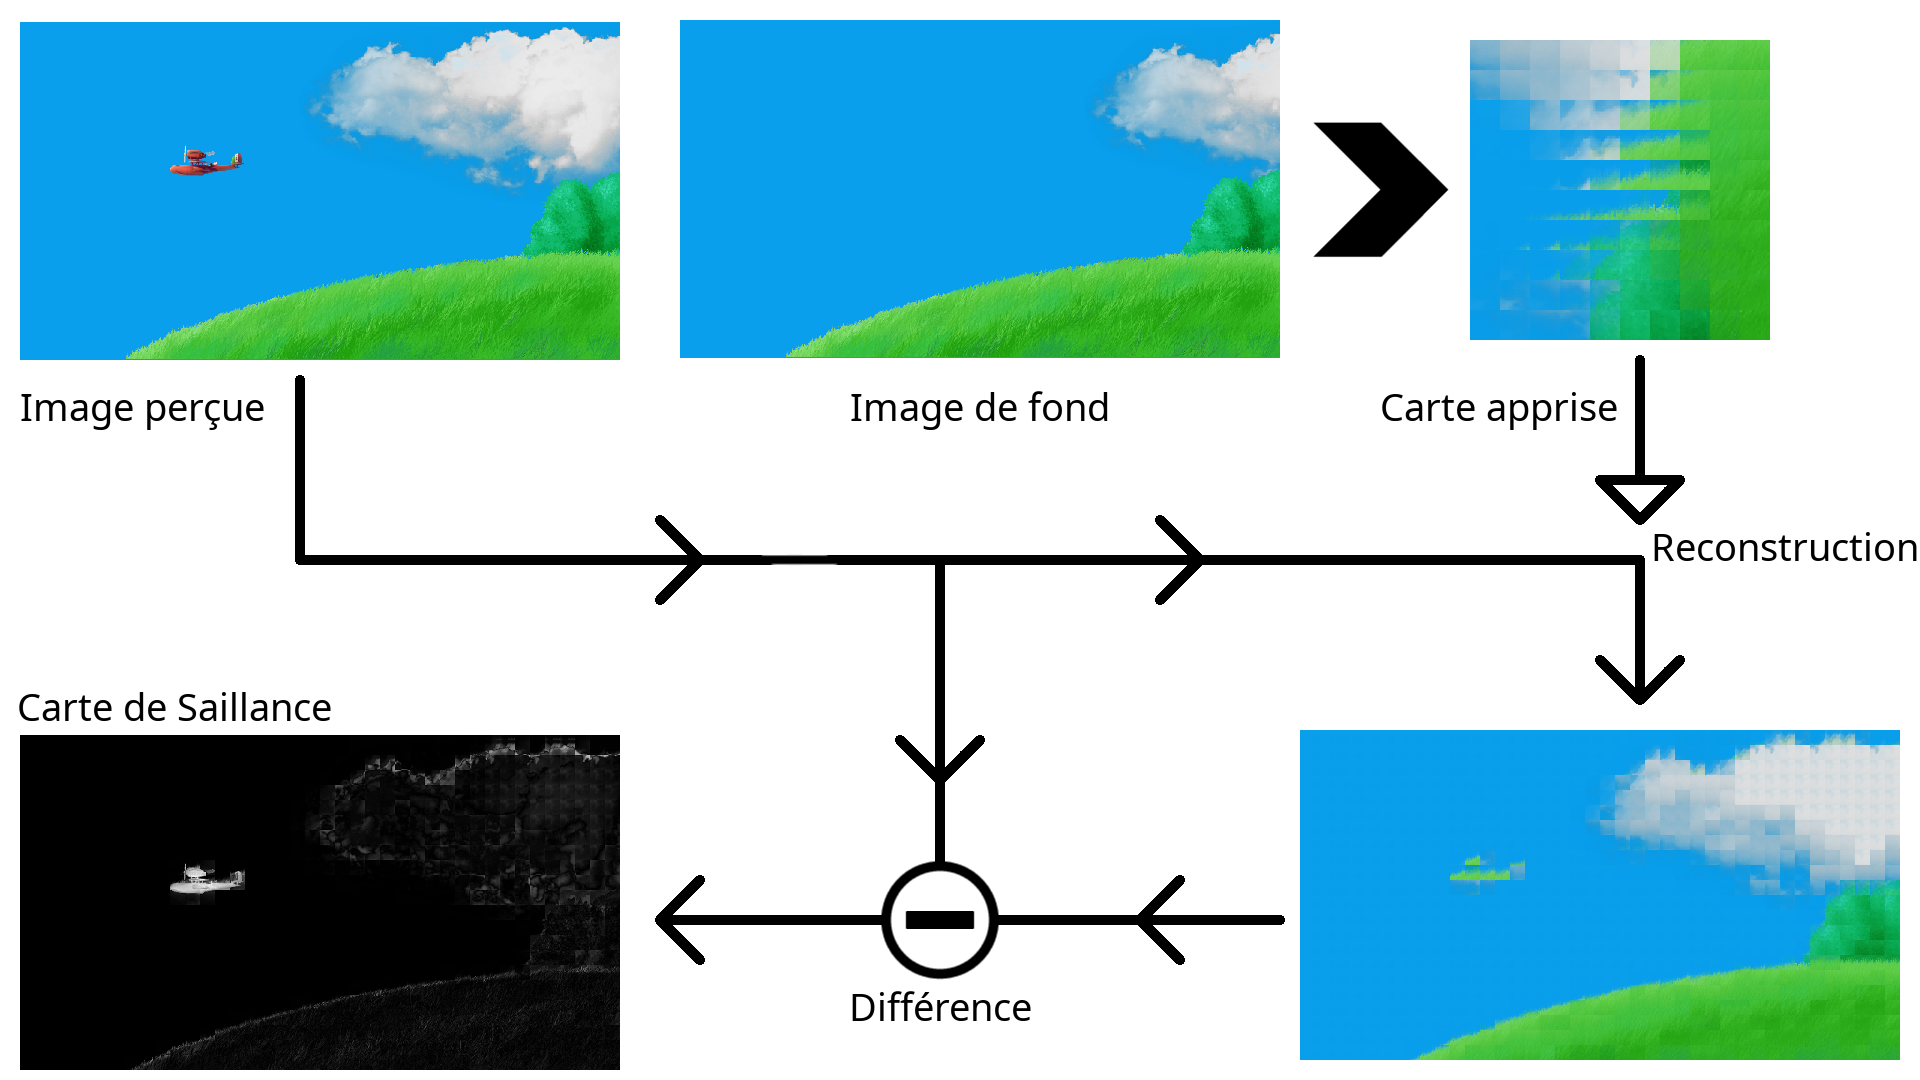
\includegraphics[width=\linewidth]{saliency_map_generation}
		\caption[Détection de nouveauté avec QV]{Fonctionnement schématique de la détection de nouveauté avec quantification vectorielle.}\label{fig:img:vq}
	\end{figureth}

	\subsection{Détection avec distance neurale}

	\begin{figureth}
		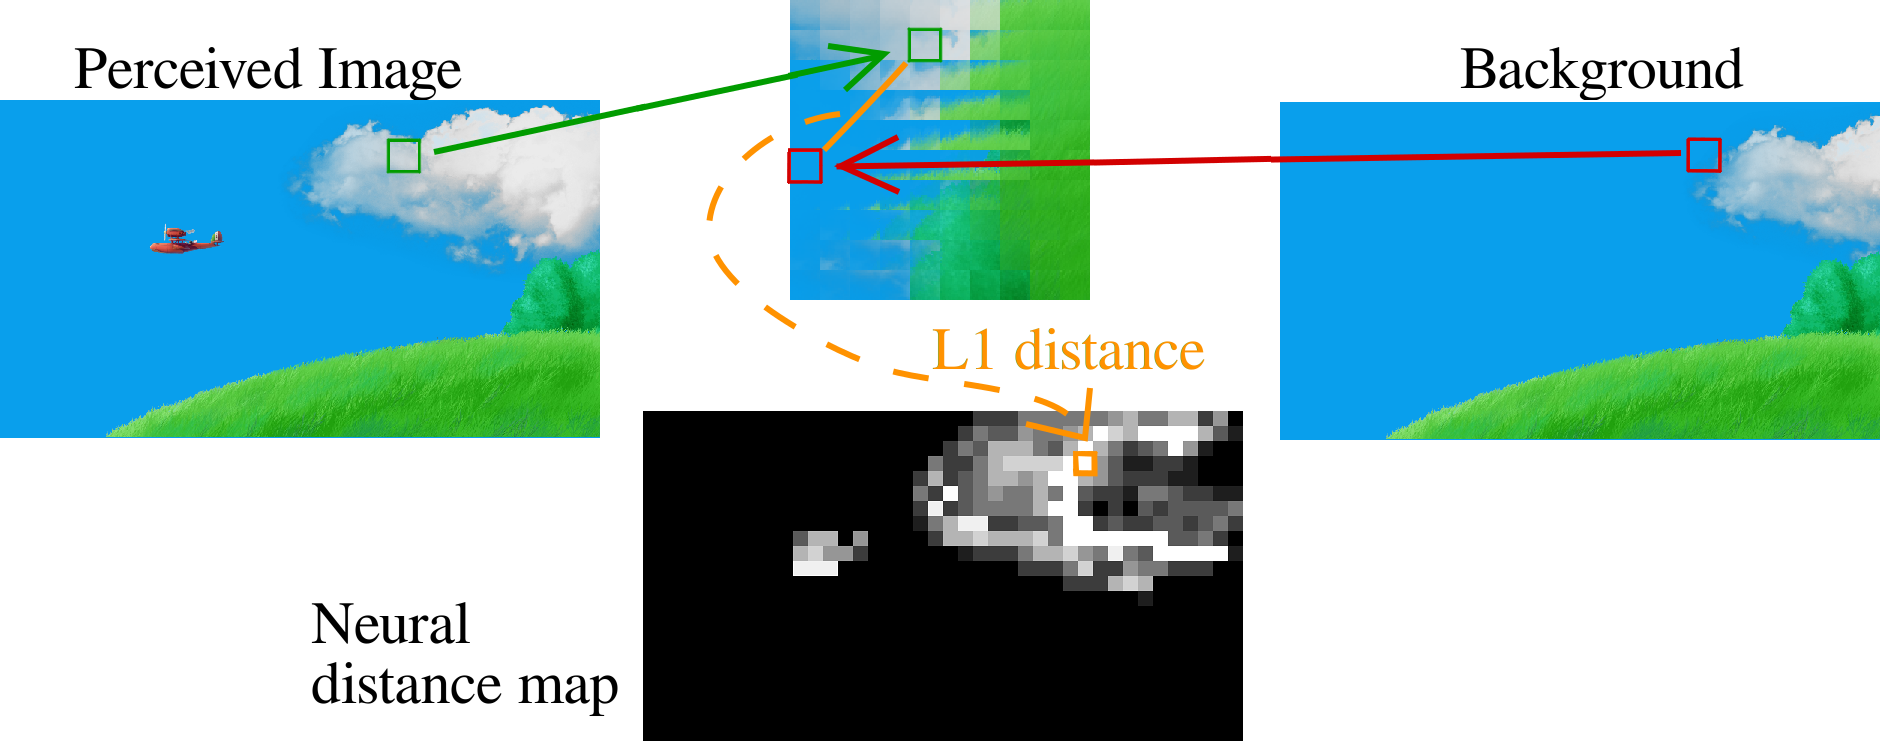
\includegraphics[width=\linewidth]{neural_distance_modulation_v2}
		\caption[Détection de nouveauté avec topologie]{Fonctionnement schématique de la détection de nouveauté avec topologie.}\label{fig:img:topo}
	\end{figureth}

	

	\subsection{Considérations pour la combinaison}
	
	Une fois les deux cartes de saillance générées, il est nécessaire de les combiner pour n'avoir qu'un seul résultat qui représentera la sortie de notre système. Il existe un très grand nombre de façons de le faire cette combinaison, et il existe dans la littérature des modèles qui se basent sur une bonne combinaison de différentes cartes de saillance pour obtenir de meilleurs résultats \nocite{todo}. Dans notre cas, nous avons avons préféré utiliser une combinaison simple de nos deux cartes de saillance. C'est à dire qu'elle n'utilise pas de paramètres (pour ne pas ajouter encore une variable à optimiser). Nous souhaitons aussi bénéficier de la complémentarité des deux cartes de saillances que l'on a. Par conséquent la solution la plus simple est de multiplier les deux cartes ensemble. Ainsi, sera considéré comme nouveauté dans la carte de sortie, ce qui apparaît comme nouveauté en même temps dans les deux cartes de saillance (car $\textit{petit} \times \textit{petit} = \textit{petit}$, $\textit{grand} \times \textit{petit} = \textit{petit}$ et seulement $\textit{grand} \times \textit{grand} = \textit{grand}$). De cette façon, le bruit qui est présent dans la carte résultant de la quantification vectorielle et qui n'est pas présent dans la carte topologique disparaît de la carte finale. Il en va de même pour les mouvements qui ne sont pas des nouveautés qui apparaissent dans la carte topologique, mais pas dans la carte de quantification vectorielle.

	Un problème qui peut apparaître dans ce cas est la trop petite valeur du résultat et le déséquilibre d'impact de nos deux cartes, car nos cartes de saillance sont toutes les deux définies entre 0 et 1. Il est possible que des situations arrivent lors desquelles les deux cartes ont un impact disproportionnel sur le résultat (par exemple si l'objet à détecter sur une carte a une valeur de 0.2 sur une carte et 0.8 sur l'autre, alors la seconde aura plus d'impact sur les valeurs de la sortie finale). De même, en multipliant deux nombres compris entre 0 et 1, le résultat sera forcément inférieur à chacun des deux nombres. Ainsi, on a aussi un effet qui réduit toutes les valeurs de la carte de saillance finale, ce qui peut poser problème si l'on n'y fait pas attention. La solution que nous avons choisi à ces des problèmes, est de re-normaliser les deux cartes de saillances avant de les multiplier. C'est à dire que l'on rééchelonne l'ensemble de la carte en mettant la valeur maximum de la carte à 1 et le minimum à 0 et d'étaler les valeurs intermédiaires entre les deux pour conserver le même espacement relatif entre elles. Cela a pour effet d'éviter une trop grande disproportion d'impact entre les deux cartes (mais ne résoud pas complètement le problème, car on re-normalise avec le maximum, et non avec la possible valeur de la nouveauté detectée), et permet d'avoir un résultat avec des valeurs généralement plus hautes. Cependant, cela vient aussi avec des désavantages, comme par exemple le fait que si il n'y a pas de signal dans l'entrée, le maximum des cartes de saillance sera quand même 1 et on pourrait observer des signaux positifs dans la sortie alors que l'entrée et les cartes de saillances n'en montrent pas. En pratique, cela est peu fréquent car la valeur maximum dans un cas où il n'y a pas de signal en entrée vient du bruit, et est donc décorellée entre les deux cartes. De plus, la taille du signal d'entrée compte, et il est peu probable que du bruit seul puisse créer une zone de signal assez large pour être confondu avec une vraie nouveauté.

	\newpage
	\section{Protocole expérimental}

	Cette section regroupe l'ensemble des considérations pratiques pour la réalisation de nos expériences. Nous présenterons la base de donnée utilisée, comment ces données ont été préparées, les différentes métriques que nous avons mesuré et les paramétrages de nos modèles.

	\subsection{Présentation de la base de données}

	Il n'existe pas à notre connaissance de base de données de détection de nouveauté respectant nos hypothèses de caméra statique, de [...]. Une alternative se trouve dans la base de donnée CDnet \cite{wang-cdnet}. Elle a pour objectif d'uniformiser les résultats dans un domaine proche de la détection de nouveauté ; la détection de changement. Les deux domaines peuvent sembler similaires au premier abord car les deux approches visent la même application réelle. Cependant cela cache une différence conceptuelle. La détection de changement se concentre sur le mouvement pour séparer le fond des objets intéressants dans une image. La détection de nouveauté quand à elle se réfère à une représentation apprise de l'environnement (discuté plus en détail dans la section [...]). Dans les captures vidéos réelles, les deux sont généralement équivalents dû au fait que lorsqu'une nouveauté apparaît, elle le fait généralement en se déplaçant. En pratique cela veut dire que la majorité de CDnet peut être utilisé pour de la détection de nouveauté. Nous présenterons les catégories et vidéos qui ont été retenues, et celles qui ont été filtrées dans la suite.
	
	CDnet regroupe 53 séquences vidéos provenant de sources variées. Elles proviennent principalement de caméras de surveillance ou de captures effectuées par des chercheurs pour leur propres besoins. Elles sont toutes des captures en couleur (sauf pour deux catégories \textit{thermal} et \textit{turbulences}) et de résolution assez faible (allant de $320 \times 240$ de $720 \times 486$ pixels). Elles sont groupées en 11 catégories de 4 à 6 vidéos sensées représenter une variété de difficultés que peuvent rencontrer les modèles de détection de changement. Ces catégories sont présentées dans les figures suivantes :

	\begin{figureth}
		\begin{subfigureth}{0.24\textwidth}
			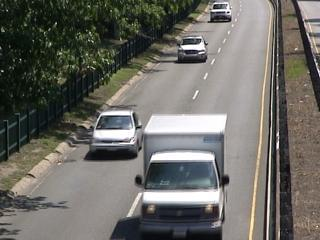
\includegraphics[width=\linewidth]{CDNET/baseline/in000277}\caption{Highway}	
		\end{subfigureth}
		\begin{subfigureth}{0.24\textwidth}
			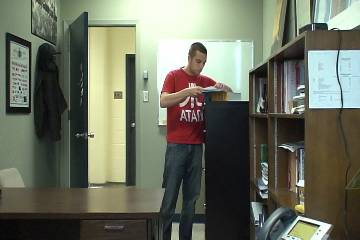
\includegraphics[width=\linewidth]{CDNET/baseline/in000895}\caption{Office}	
		\end{subfigureth}
		\begin{subfigureth}{0.24\textwidth}
			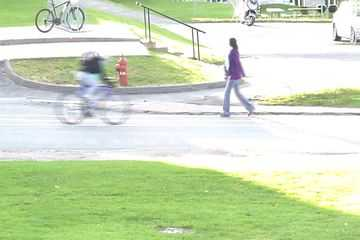
\includegraphics[width=\linewidth]{CDNET/baseline/in000473}\caption{Pedestrians}	
		\end{subfigureth}
		\begin{subfigureth}{0.24\textwidth}
			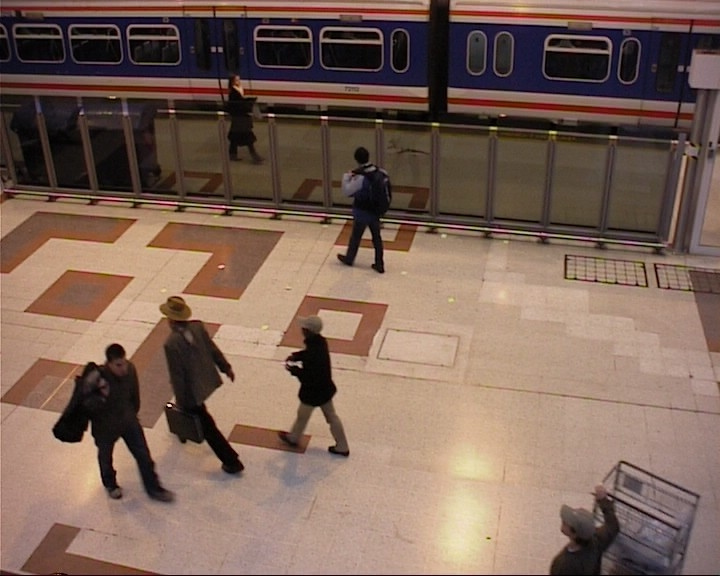
\includegraphics[width=\linewidth]{CDNET/baseline/in000118}\caption{PETS2006}	
		\end{subfigureth}
		\caption[Catégorie Baseline]{\textit{Baseline} : La catégorie de base qui comprend des scénarios typiques de détection de changement (traffic, piétons) sans difficultés particulières.}\label{fig:cdnet:baseline}
	\end{figureth}

	\begin{figureth}
		\begin{subfigureth}{0.24\textwidth}
			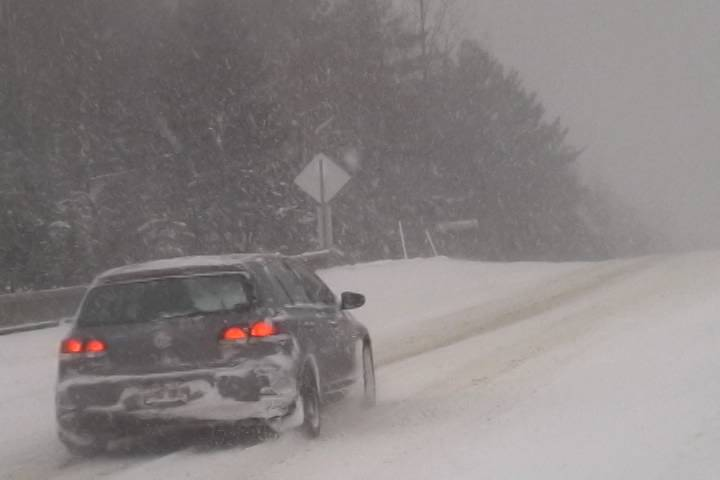
\includegraphics[width=\linewidth]{CDNET/badWeather/in000810}\caption{Snowfall}	
		\end{subfigureth}
		\begin{subfigureth}{0.24\textwidth}
			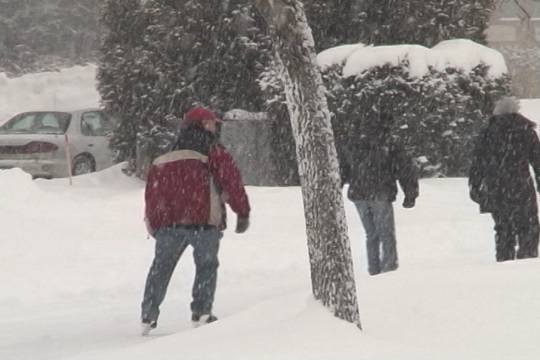
\includegraphics[width=\linewidth]{CDNET/badWeather/in001951}\caption{Skating}	
		\end{subfigureth}
		\begin{subfigureth}{0.24\textwidth}
			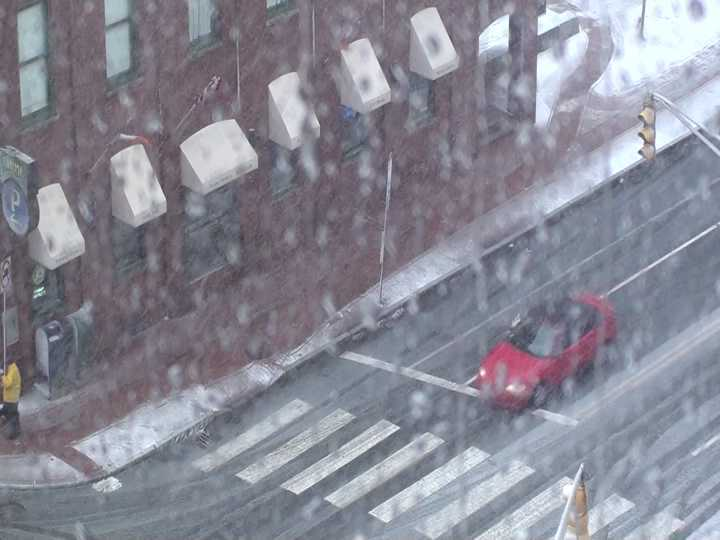
\includegraphics[width=\linewidth]{CDNET/badWeather/in002841}\caption{WetSnow}	
		\end{subfigureth}
		\begin{subfigureth}{0.24\textwidth}
			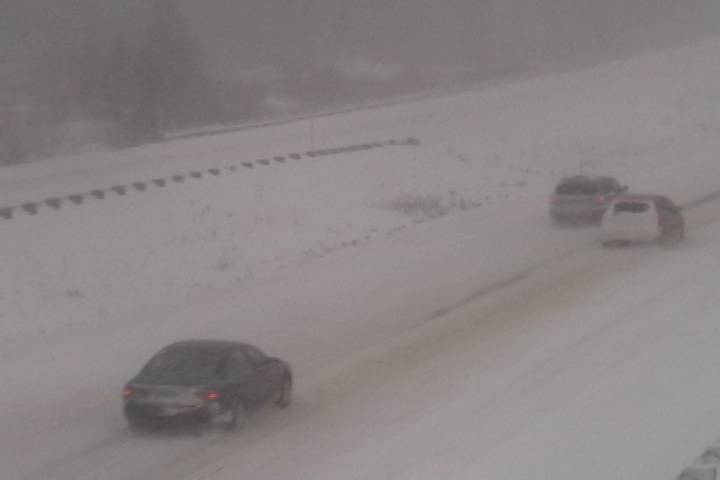
\includegraphics[width=\linewidth]{CDNET/badWeather/in004863}\caption{Blizzard}	
		\end{subfigureth}
		\caption[Catégorie Bad weather]{\textit{Bad weather} : Cette catégorie comprend des variations du scénario de base avec une météo dégradée. La difficulté principale vient de la neige qui tombe, et du changment de l'environnement avec les traces de pneus sur la neige par exemple.}\label{fig:cdnet:badweather}
	\end{figureth}

	\begin{figureth}
		\begin{subfigureth}{0.24\textwidth}
			\includegraphics[width=\linewidth]{CDNET/cameraJitter/in000145}\caption{Sidewalk}	
		\end{subfigureth}
		\begin{subfigureth}{0.24\textwidth}
			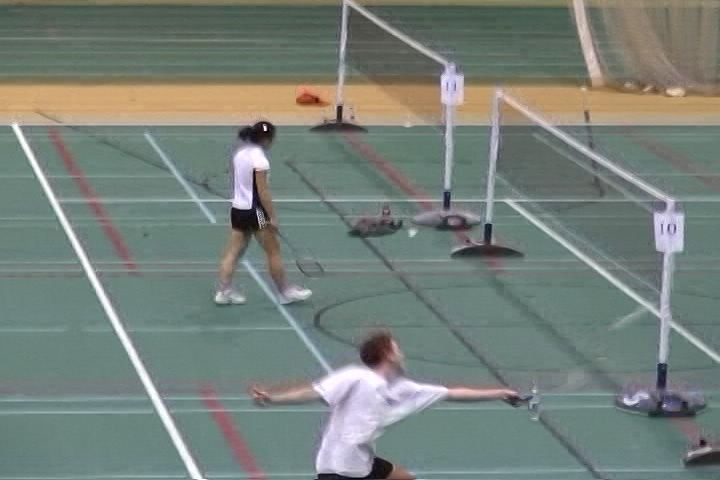
\includegraphics[width=\linewidth]{CDNET/cameraJitter/in000187}\caption{Badminton}	
		\end{subfigureth}
		\begin{subfigureth}{0.24\textwidth}
			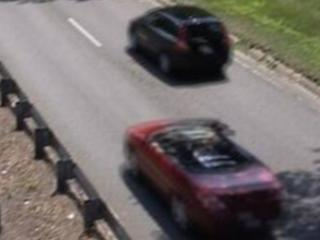
\includegraphics[width=\linewidth]{CDNET/cameraJitter/in000355}\caption{Traffic}	
		\end{subfigureth}
		\begin{subfigureth}{0.24\textwidth}
			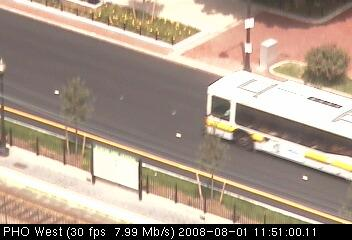
\includegraphics[width=\linewidth]{CDNET/cameraJitter/in002287}\caption{Boulevard}	
		\end{subfigureth}
		\caption[categorie camera jitter]{\textit{Camera Jitter} : Ces vidéos proviennent de caméras instables à cause de vent fort ou d'autres raisons. Elles ont de façon irrégulière des translations verticales et horizontales  rapides et de petite amplitude.}\label{fig:cdnet:jitter}
	\end{figureth}

	\begin{figureth}
		\begin{subfigureth}{0.24\textwidth}
			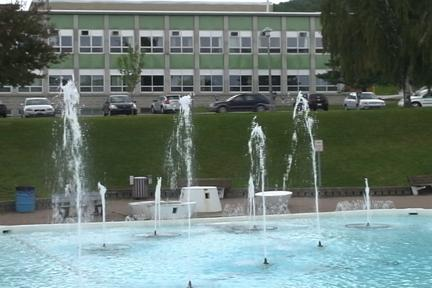
\includegraphics[width=\linewidth]{CDNET/dynamicBackground/in000716}\caption{Fountain01}	
		\end{subfigureth}
		\begin{subfigureth}{0.24\textwidth}
			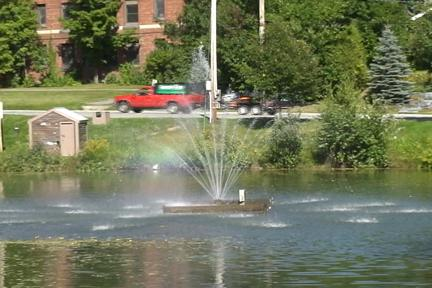
\includegraphics[width=\linewidth]{CDNET/dynamicBackground/in000720}\caption{Fountain02}	
		\end{subfigureth}
		\begin{subfigureth}{0.24\textwidth}
			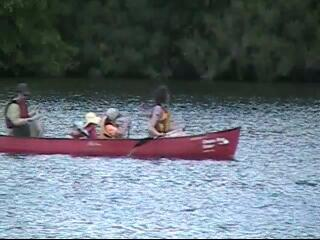
\includegraphics[width=\linewidth]{CDNET/dynamicBackground/in000937}\caption{Canoe}	
		\end{subfigureth}\\
		\begin{subfigureth}{0.24\textwidth}
			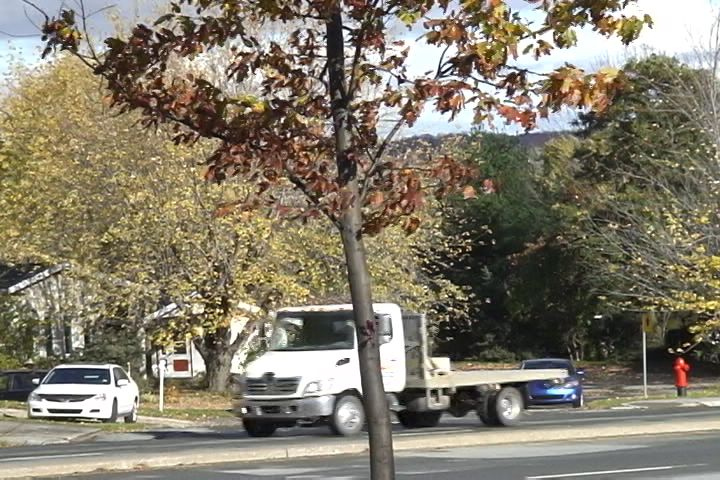
\includegraphics[width=\linewidth]{CDNET/dynamicBackground/in001504}\caption{Fall}	
		\end{subfigureth}
		\begin{subfigureth}{0.24\textwidth}
			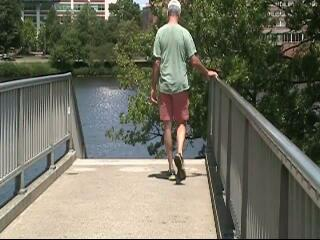
\includegraphics[width=\linewidth]{CDNET/dynamicBackground/in002519}\caption{Overpass}	
		\end{subfigureth}
		\begin{subfigureth}{0.24\textwidth}
			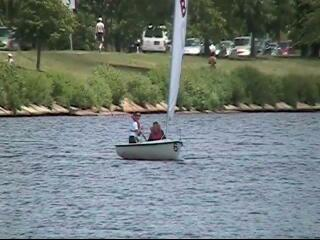
\includegraphics[width=\linewidth]{CDNET/dynamicBackground/in007726}\caption{Boats}	
		\end{subfigureth}
		\caption[Categorie Dynamic Background]{\textit{Dynamic Background} : La difficulté se porte sur le contenu du fond qui est changeant. Il peut s'agir d'eau ou d'arbres qui bougent dans le vent.}\label{fig:cdnet:dynamic}
	\end{figureth}

	\begin{figureth}
		\begin{subfigureth}{0.24\textwidth}
			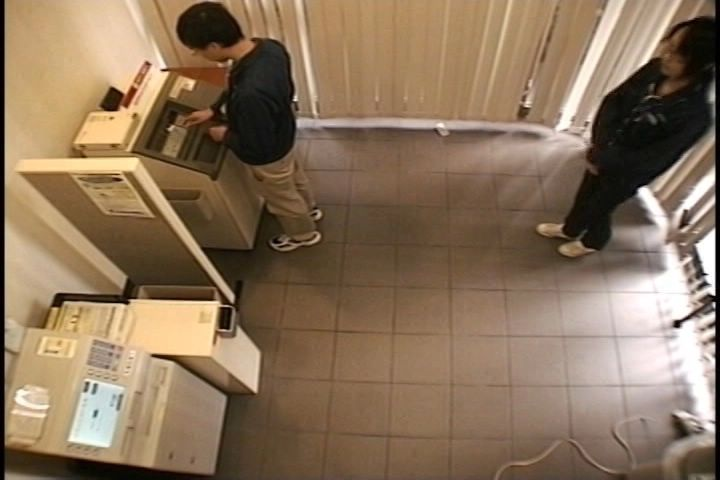
\includegraphics[width=\linewidth]{CDNET/shadow/in000260}\caption{CopyMachine}
		\end{subfigureth}
		\begin{subfigureth}{0.24\textwidth}
			\includegraphics[width=\linewidth]{CDNET/shadow/in000320}\caption{PeopleInShade}
		\end{subfigureth}
		\begin{subfigureth}{0.24\textwidth}
			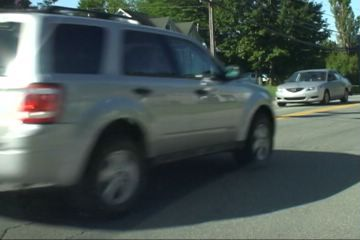
\includegraphics[width=\linewidth]{CDNET/shadow/in000358}\caption{Bungalows}	
		\end{subfigureth}\\
		\begin{subfigureth}{0.24\textwidth}
			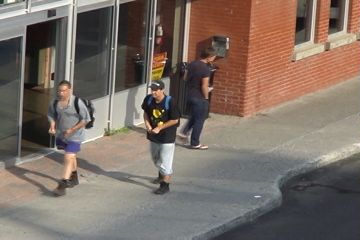
\includegraphics[width=\linewidth]{CDNET/shadow/in001015}\caption{BusStation}	
		\end{subfigureth}
		\begin{subfigureth}{0.24\textwidth}
			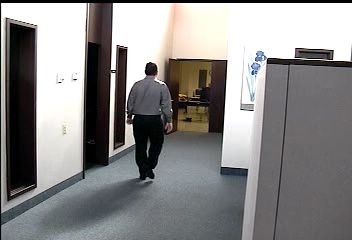
\includegraphics[width=\linewidth]{CDNET/shadow/in001210}\caption{Cubicle}
		\end{subfigureth}
		\begin{subfigureth}{0.24\textwidth}
			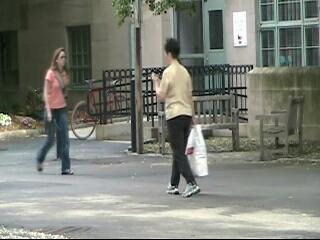
\includegraphics[width=\linewidth]{CDNET/shadow/in001850}\caption{Backdoor}	
		\end{subfigureth}
		\caption[Categorie Shadow]{\textit{Shadow} : Catégorie de vidéos qui présente plus d'ombres que la moyenne.}\label{fig:cdnet:shadow}
	\end{figureth}

	\begin{figureth}
		\begin{subfigureth}{0.24\textwidth}
			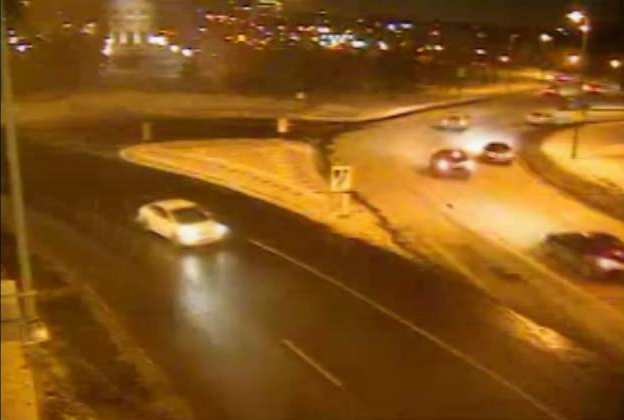
\includegraphics[width=\linewidth]{CDNET/nightVideos/in000060}\caption{WinterStreet}	
		\end{subfigureth}
		\begin{subfigureth}{0.24\textwidth}
			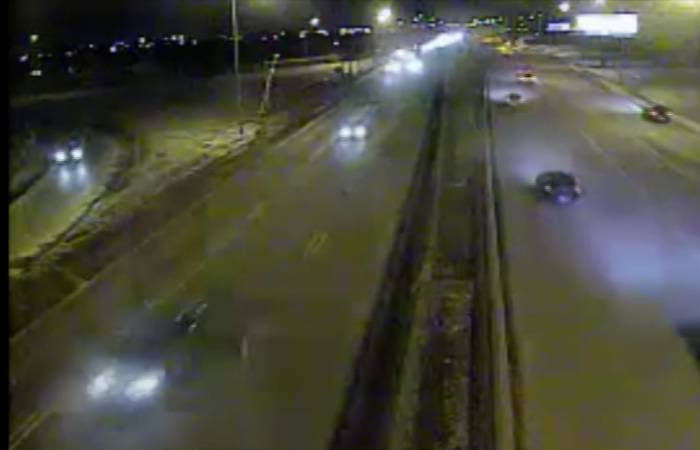
\includegraphics[width=\linewidth]{CDNET/nightVideos/in000125}\caption{FluidHighway}	
		\end{subfigureth}
		\begin{subfigureth}{0.24\textwidth}
			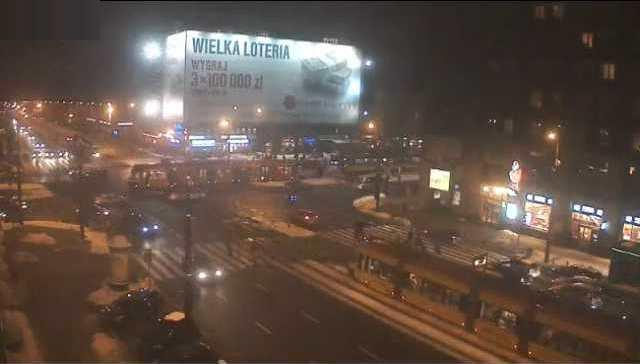
\includegraphics[width=\linewidth]{CDNET/nightVideos/in000150}\caption{BusyBoulevard}	
		\end{subfigureth}\\
		\begin{subfigureth}{0.24\textwidth}
			\includegraphics[width=\linewidth]{CDNET/nightVideos/in000320}\caption{TramStation}	
		\end{subfigureth}
		\begin{subfigureth}{0.24\textwidth}
			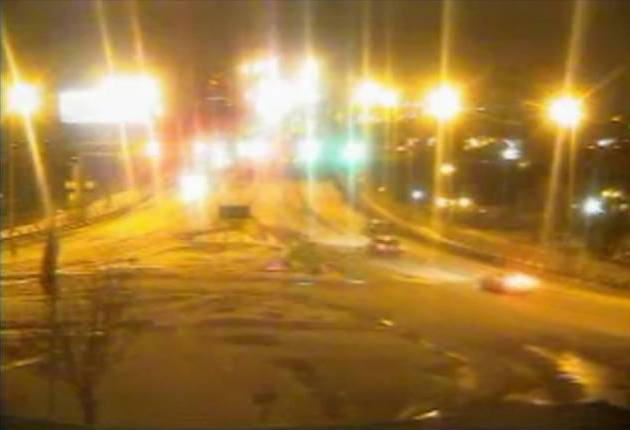
\includegraphics[width=\linewidth]{CDNET/nightVideos/in000362}\caption{BridgeEntry}	
		\end{subfigureth}
		\begin{subfigureth}{0.24\textwidth}
			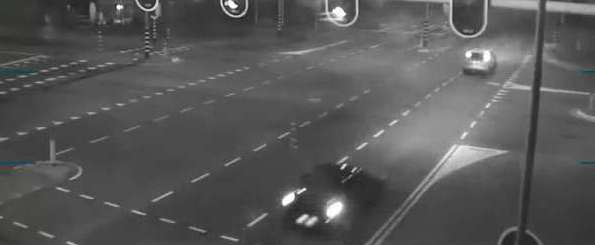
\includegraphics[width=\linewidth]{CDNET/nightVideos/in000671}\caption{StreetCornerAtNight}	
		\end{subfigureth}
		\caption[Categorie Night Videos]{\textit{Night Videos} : Vidéos de nuit avec un contraste fort entre l'obscurité ambiante et les lumières artificielles de l'éclairage public et des phares de voitures.}\label{fig:cdnet:night}
	\end{figureth}

	\begin{figureth}
		\begin{subfigureth}{0.24\textwidth}
			\includegraphics[width=\linewidth]{CDNET/thermal/in000145}\caption{Park}
		\end{subfigureth}
		\begin{subfigureth}{0.24\textwidth}
			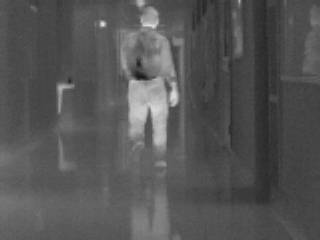
\includegraphics[width=\linewidth]{CDNET/thermal/in000800}\caption{Corridor}	
		\end{subfigureth}
		\begin{subfigureth}{0.24\textwidth}
			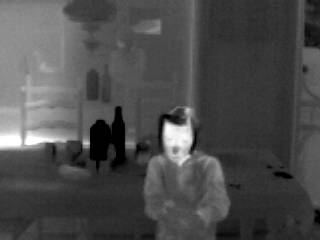
\includegraphics[width=\linewidth]{CDNET/thermal/in000840}\caption{DiningRoom}	
		\end{subfigureth}\\
		\begin{subfigureth}{0.24\textwidth}
			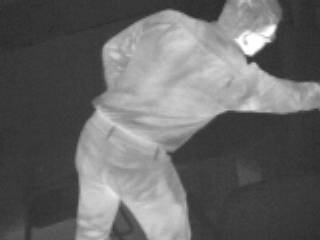
\includegraphics[width=\linewidth]{CDNET/thermal/in001050}\caption{Library}	
		\end{subfigureth}
		\begin{subfigureth}{0.24\textwidth}
			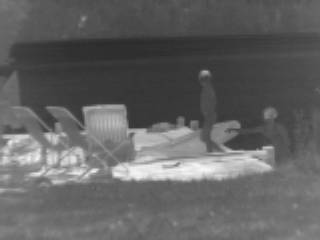
\includegraphics[width=\linewidth]{CDNET/thermal/in002220}\caption{LakeSide}	
		\end{subfigureth}
		\caption[Categorie thermal]{\textit{Thermal} : Ces vidéos ont été prises par une caméra infrarouge et sont en niveau de gris.}\label{fig:cdnet:shadow}
	\end{figureth}

	\begin{figureth}
		\begin{subfigureth}{0.24\textwidth}
			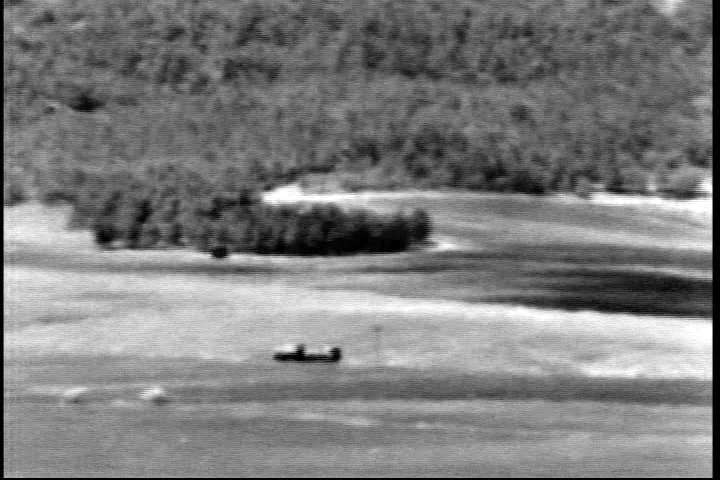
\includegraphics[width=\linewidth]{CDNET/turbulence/in000425}\caption{Turbulence0}	
		\end{subfigureth}
		\begin{subfigureth}{0.24\textwidth}
			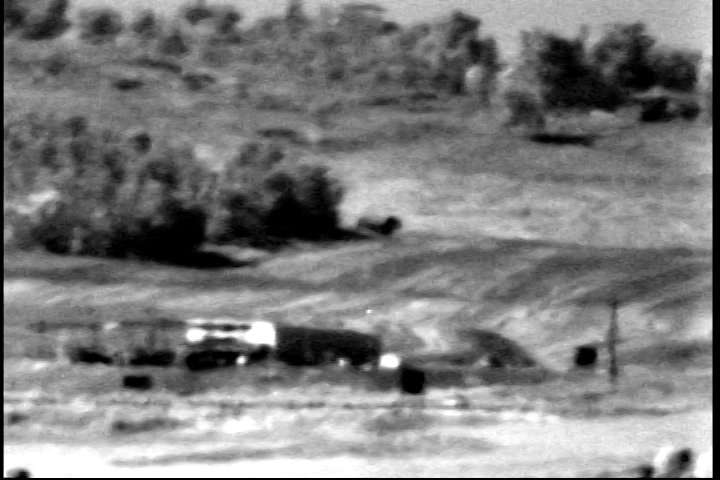
\includegraphics[width=\linewidth]{CDNET/turbulence/in000920}\caption{Turbulence1}	
		\end{subfigureth}
		\begin{subfigureth}{0.24\textwidth}
			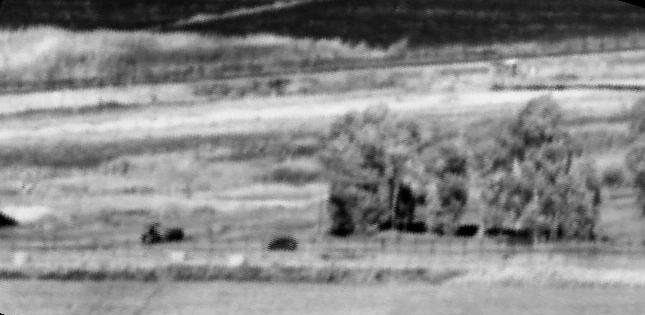
\includegraphics[width=\linewidth]{CDNET/turbulence/in000140}\caption{Turbulence2}	
		\end{subfigureth}
		\begin{subfigureth}{0.24\textwidth}
			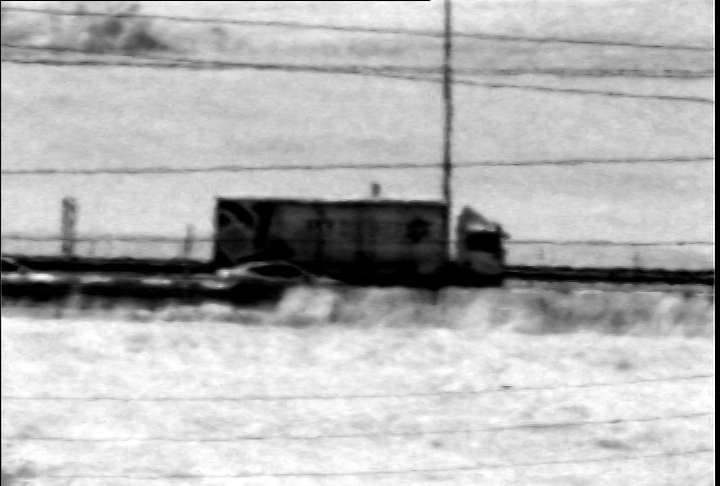
\includegraphics[width=\linewidth]{CDNET/turbulence/in000195}\caption{Turbulence3}	
		\end{subfigureth}
		\caption[Categorie turbulence]{\textit{Turbulence} : Catégorie qui regroupe des vidéos provenant d'une même caméra infrarouge. Les captures ont été faites avec un objectif longue distance filmant des scènes à 5 à 15 km de l'objectif. Elle présente de nombreuses distortions et turbulences atmosphérique dûs à la chaleur et à la distance.}\label{fig:cdnet:turbulence}
	\end{figureth}
	
	\begin{figureth}
		\begin{subfigureth}{0.24\textwidth}
			\includegraphics[width=\linewidth]{CDNET/intermittentObjectMotion/in001000}\caption{StreetLight}
		\end{subfigureth}
		\begin{subfigureth}{0.24\textwidth}
			\includegraphics[width=\linewidth]{CDNET/intermittentObjectMotion/in001300}\caption{Sofa}	
		\end{subfigureth}
		\begin{subfigureth}{0.24\textwidth}
			\includegraphics[width=\linewidth]{CDNET/intermittentObjectMotion/in001350}\caption{Tramstop}	
		\end{subfigureth}
		\caption[Categorie intermittent object motion - Reduced]{\textit{Intermittent object motion Reduced} : Cette catégorie comprend des scénarios particuliers dans lesquels le changement est intermittent (c'est à dire qu'un objet passe de mouvement à statique ou inversement). Dans cette catégorie trois vidéos sur six on été conservées.}\label{fig:cdnet:shadow}
	\end{figureth}

	\begin{figureth}
		\begin{subfigureth}{0.24\textwidth}
			\includegraphics[width=\linewidth]{CDNET/lowFramerate/in000062}\caption{Turnpike}	
		\end{subfigureth}
		\begin{subfigureth}{0.24\textwidth}
			\includegraphics[width=\linewidth]{CDNET/lowFramerate/in000088}\caption{TramCrossroad}	
		\end{subfigureth}
		\begin{subfigureth}{0.24\textwidth}
			\includegraphics[width=\linewidth]{CDNET/lowFramerate/in000235}\caption{Tunnel Exit}	
		\end{subfigureth}
		\caption[Categorie low framerate - Reduced]{\textit{Low Framerate Reduced} : Cette catégorie regroupe des vidéos avec beaucoup de temps entre les images (entre 1 seconde et 6 seconde entre chaque image). Cela a pour but de pénaliser les approches à partir de flow optique, cependant notre approche n'est pas concernée. Trois vidéos sur les quatre ont été conservées. Seule une vidéo d'une marina a été retirée car la nouveauté (des bateaux) était trop similaire au fond, qui consiste en un grand nombre de bateaux ammarés.}\label{fig:cdnet:fps}
	\end{figureth}


	Reduced categories explanations.

	\begin{figureth}
		\begin{subfigureth}{0.24\textwidth}
			\includegraphics[width=\linewidth]{intermittentObjectExample/in001285}\caption{Highway}	
		\end{subfigureth}
		\begin{subfigureth}{0.24\textwidth}
			\includegraphics[width=\linewidth]{intermittentObjectExample/gt001285}\caption{Office}	
		\end{subfigureth}
		\begin{subfigureth}{0.24\textwidth}
			\includegraphics[width=\linewidth]{intermittentObjectExample/in001815}\caption{Pedestrians}	
		\end{subfigureth}
		\begin{subfigureth}{0.24\textwidth}
			\includegraphics[width=\linewidth]{intermittentObjectExample/gt001815}\caption{PETS2006}	
		\end{subfigureth}
		\caption[camera jitter category]{Shadows}\label{fig:cdnet:shadow}
	\end{figureth}

	
	Il y a aussi dans également deux catégories que nous avons décidé de ne pas du tout utiliser car elles ne correspondent pas à notre scénario. \textit{Pan tilt zoom} : Catégorie un peu spéciale car elle change une partie fondamentale du scénario. La caméra n'est plus statique mais effectue des roations et des zooms ce qui change significativement son environnement visuel. Ce qui ne colle pas avec notre scénario.

	\subsection{Métriques utilisées}

	CDNET fournit un ensemble de métriques pour évaluer et se comparer à d'autres modèles. On s'est limité à 3 qui sont les plus pertinentes, les autres étant secondaires à notre goût.

	\subsubsection{QE : Quantization Error}

	Basé sur la somme des distances entre les entrées et les winner. Formule. Simple à calculer. Egal à la distance calculée pour déterminer les gagnants. Par conséquent valeur qu'optimise notre modèle. Cependant mauvaise graduation des résultats. La non pénalisation des outliers peut être problématique par exemple.

	\subsubsection{PSNR : Peak Signal to Noise Ratio}

	Similaire à QE, mais avec un carré. Très présent dans la littérature. Formule. Logarithme pour plus de lisibilité. Moins de problèmes avec outliers mais toujours beaucoup de problèmes de bonne échelle de différence.

	\subsubsection{Précision}

	Mesure classique et très connue. Formule. Explication de ce que ça mesure.

	\subsubsection{Rappel}

	Mesure classique et très connue. Formule. Explication de ce que ça mesure.

	\subsubsection{F-measure}

	Mesure un peu plus complexe qui essaye de regrouper Prec et rappel en un nombre. Formule. Explication comportement en fonction de precision et rappel.

	\subsubsection{Oeil humain Mk. 1}

	Trouver une métrique correcte serait trop complexe et reviendrait à résoudre le problème initial de toutes façons. Par conséquent utiliser l'oeil humain pour analyser les résultats peut parfois donner la meilleure interprétation de ce qu'il se passe. Particulièrement intéressant pour comparer différentes méthodes entre elles.

	\subsection{Préparation des données}

	Parfois, nouveauté dès le début de la capture. Médiane des X premières images pour obtenir des fond sans nouveauté. Peut parfois lisser les intempéries (figure). Mais pas d'impact sur les résultats (tableau à l'appui). Utilisation d'une partie seulement de la CDNET (1 image sur 50) pour evaluer plus rapidement.

	\subsection{Paramétrages des modèles}

	Liste de tous les paramètres. Les limites de chacun (max, min), leurs effets (plus de calculs, ...) différentes optimisations faites (études séparées pour les époch, alpha, sigma). Les valeurs prises pour les expériences. Tableau récapitulatif.

	\newpage

	\section{Résultats expérimentaux}
	\subsection{Evaluation de la qualité de reconstruction}

	Des graphes, pleins de graphes. Et des tableaux. Et des figures.

	\subsection{Evaluation de la détection de nouveauté}
	
	Des graphes, pleins de graphes. Et des tableaux. Et des figures.

	\subsection{Interprétations}

	Mauvaise généralisation qui empêche la caméra en mouvement. La compression est différente du tracking (meilleure compression != meilleur tracking). Problème de distances pour l'apprentissage pour correctement représenter les images.

	\section{Conclusion}
		
\bibliographystyle{francaissc}
\bibliography{Chapitre2/Biblio}